\documentclass{beamer}
\usetheme{Madrid}

\usepackage{ctex}

\title{蒙特卡罗方法}
\author{祝润天}
\institute{复旦大学计算机科学技术学院}
\date{2024 年 9 月 13 日}

\begin{document}

\begin{frame}
    
    \maketitle

\end{frame}

\section{计算圆周率}

\begin{frame}
    \frametitle{计算圆周率}

    \begin{problem}
        如何计算圆周率的具体数值?       
    \end{problem}

    \pause

    \begin{block}{级数方法}
        $$\frac{\pi}{4} = 1 - \frac{1}{3} + \frac{1}{5} - \frac{1}{7} + \frac{1}{9} - \cdots = \sum_{k = 0}^{\infty} \frac{(-1)^k}{2k + 1}$$
        $$\pi = 4\sum_{k = 0}^{\infty} \frac{(-1)^k}{2k + 1}$$
    \end{block}

\end{frame}

\begin{frame}
    \frametitle{计算圆周率}

    \begin{problem}
        如何计算圆周率的具体数值?       
    \end{problem}

    \begin{block}{楚德诺夫斯基(Chudnovsky)算法}
        $$S = \sum_{n = 0}^{\infty} (-1)^n \frac{(6n)!(k_2+nk_1)}{(n!)^3(3n)!(8k_4k_5)^n}$$
        $$\pi = \frac{k_6\sqrt{k_3}}{S}$$
        其中
        $$k_1 = 545140134, k_2 = 13591409, k_3 = 640320,$$
        $$k_4 = 100100025, k_5 = 327843840, k_6 = 53360$$
    \end{block}
    太吓人了!(也不是今天的主题)

\end{frame}

\begin{frame}
    \frametitle{投点法}

    \begin{problem}
        在边长为 $1$ 的正方形中有一内接四分之一圆。在正方形中随机取点,点在四分之一圆内的概率是多少?   
    \end{problem}

    \begin{columns}
        \column{.38\textwidth}

        \pause

        $$p = \frac{S_{\text{圆}}}{S_{\text{正方形}}} = \frac{\pi}{4}$$
    
        $$\pi = 4p$$

        \column{.58\textwidth}

        \begin{figure}
            \centering
            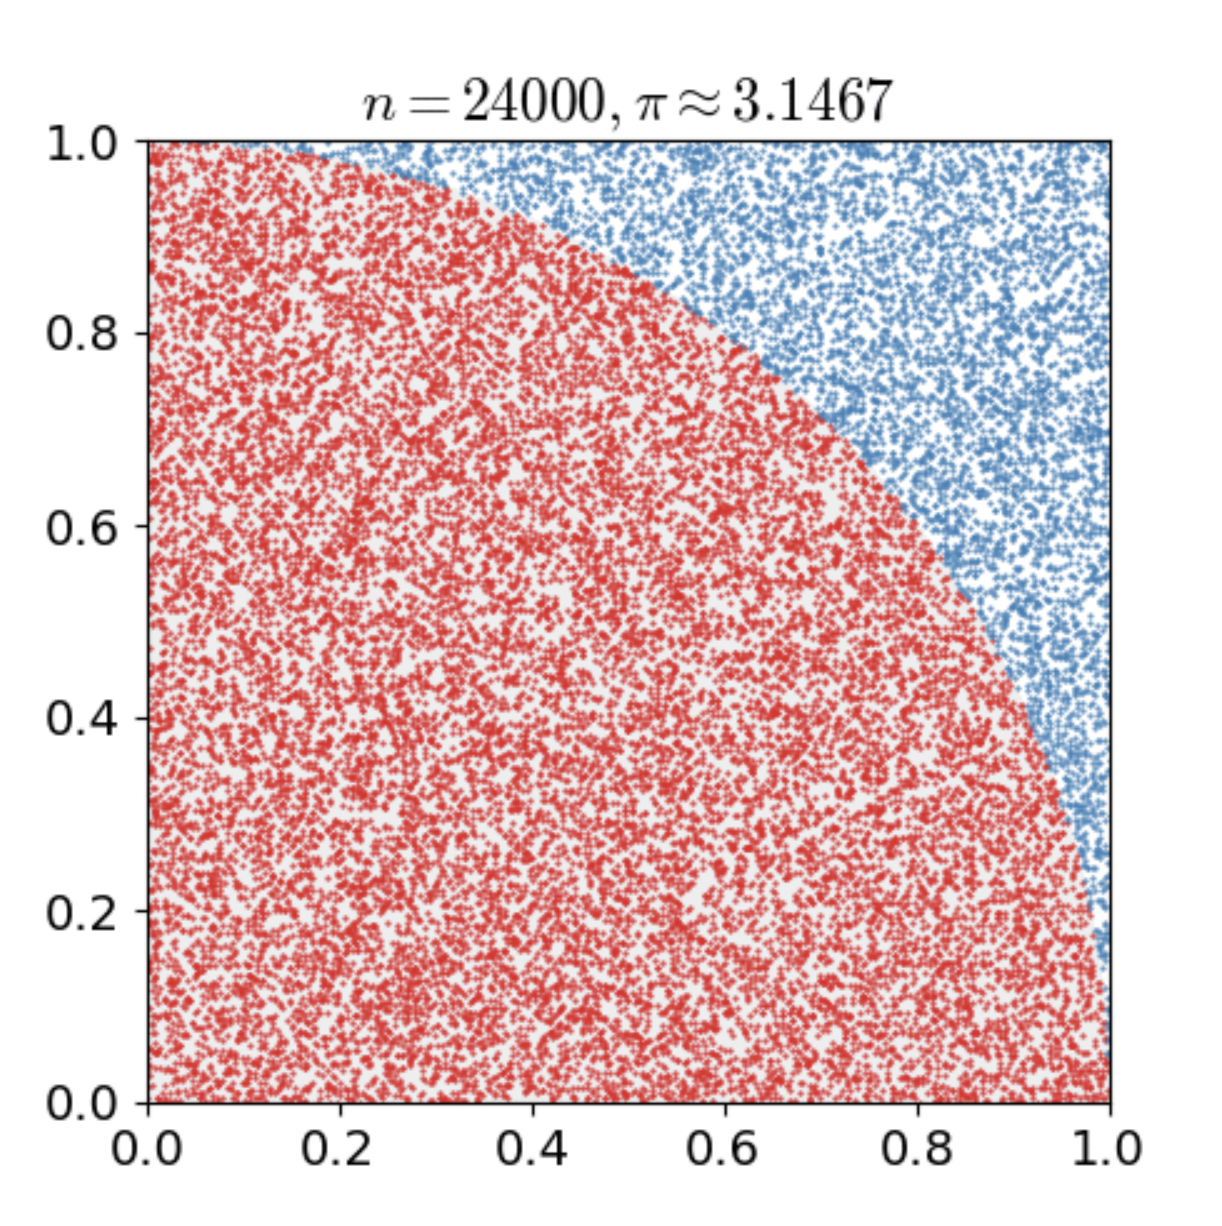
\includegraphics[scale=0.12]{res/pi_calc.png}
        \end{figure}
    \end{columns}

\end{frame}

\begin{frame}
    \frametitle{布丰投针}

    \begin{problem}
        设我们有一个以平行且等距木纹铺成的地板(如图),现在随意抛一支长度比木纹之间距离小的针,求针和其中一条木纹相交的概率。
    \end{problem}

    \begin{columns}
        \column{.48\textwidth}

        设针的长度为 $l$,平行线间距为 $t$,$x$ 为针的中心和最近的平行线的距离,$\theta$ 为针和线之间的锐角。

        $x \in [0, t/2]$ 且均匀分布;

        $\theta \in [0, \pi/2]$ 且均匀分布。

        \column{.48\textwidth}
   
        \begin{figure}
            \centering
            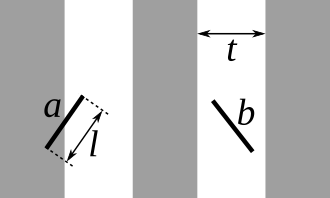
\includegraphics[width=.95\textwidth]{res/buffon.png}
        \end{figure} 
    \end{columns}

\end{frame}

\section{蒙特卡罗方法}

\begin{frame}
    \frametitle{蒙特卡罗方法}

    \begin{definition}
        通过多次随机试验,用试验得到的频率来近似计算概率。
    \end{definition}

    \begin{block}{分类}
        \begin{itemize}
            \item 所求解问题可以转化为某种随机分布的特征数。
            \begin{itemize}
                \item 利用投点法中点在圆内的概率求 $\pi$
                \item 利用布丰投针的概率求 $\pi$
            \end{itemize}
            \item 所求解的问题本身具有内在的随机性。
            \begin{itemize}
                \item 分析中子在反应堆中的传输过程
            \end{itemize}
        \end{itemize}
    \end{block}
\end{frame}

\section{应用}

\begin{frame}
    \frametitle{蒙特卡罗方法的应用}

    \begin{columns}
        \column{.48\textwidth}
        
        \begin{figure}
            \centering
            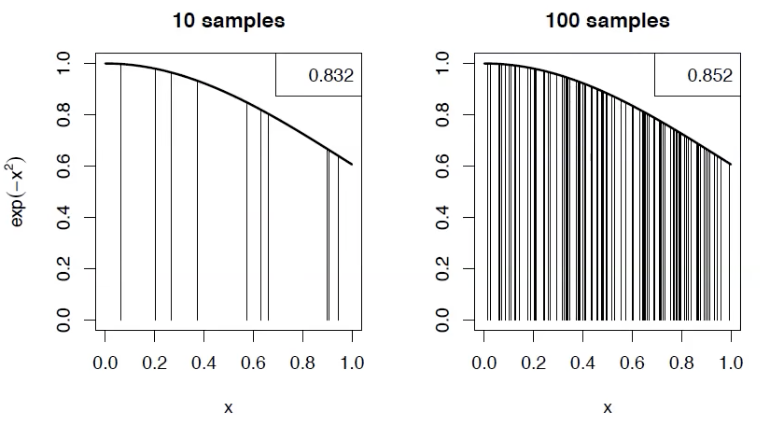
\includegraphics[width=.98\textwidth]{res/integral.png}
            \caption{计算定积分}
        \end{figure}

        \column{.48\textwidth}
        
        \begin{figure}
            \centering
            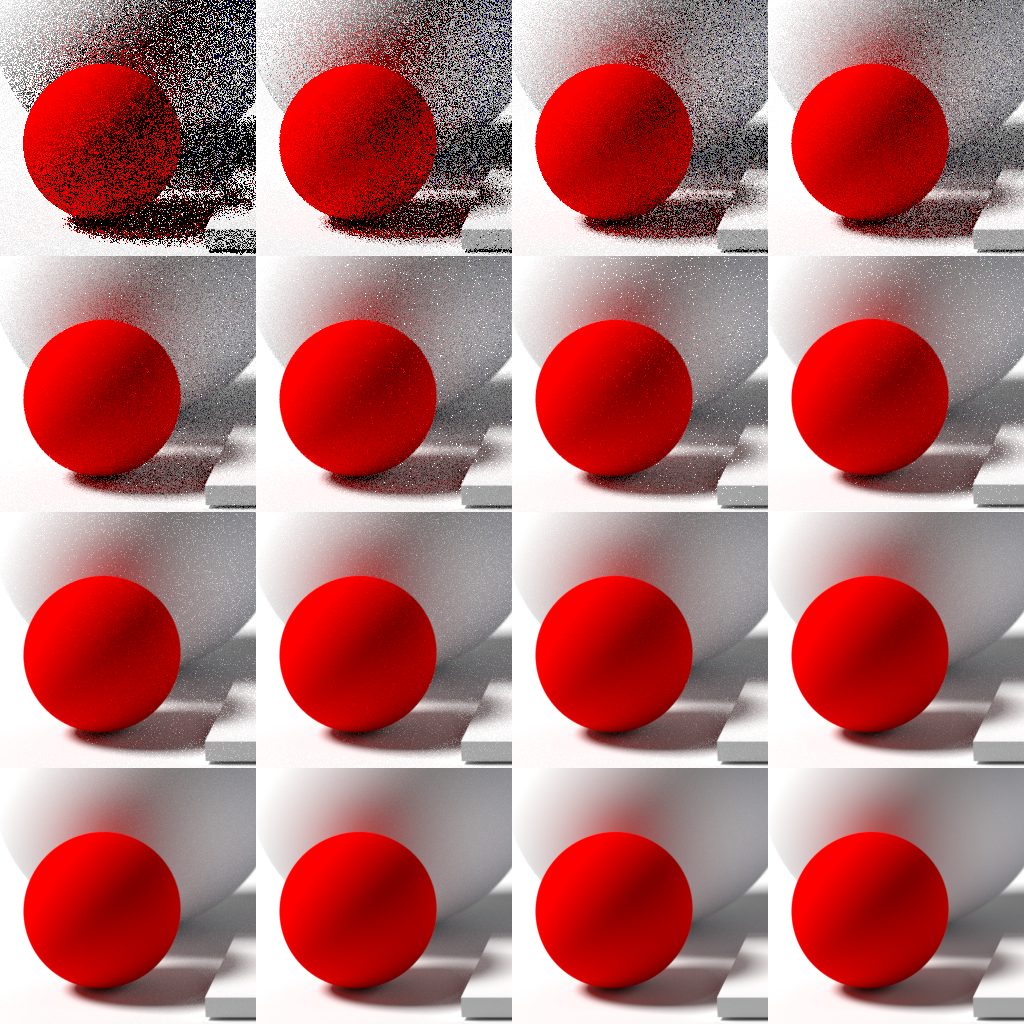
\includegraphics[width=.98\textwidth]{res/path_tracing_sampling.png}
            \caption{计算机图形学:路径追踪}
        \end{figure}
    \end{columns}
    
\end{frame}

\end{document}